\documentclass[11pt,compress,t,notes=noshow]{beamer}\usepackage[]{graphicx}\usepackage[]{color}

\makeatletter
\def\maxwidth{ %
  \ifdim\Gin@nat@width>\linewidth
    \linewidth
  \else
    \Gin@nat@width
  \fi
}
\makeatother

\definecolor{fgcolor}{rgb}{0.345, 0.345, 0.345}
\newcommand{\hlnum}[1]{\textcolor[rgb]{0.686,0.059,0.569}{#1}}%
\newcommand{\hlstr}[1]{\textcolor[rgb]{0.192,0.494,0.8}{#1}}%
\newcommand{\hlcom}[1]{\textcolor[rgb]{0.678,0.584,0.686}{\textit{#1}}}%
\newcommand{\hlopt}[1]{\textcolor[rgb]{0,0,0}{#1}}%
\newcommand{\hlstd}[1]{\textcolor[rgb]{0.345,0.345,0.345}{#1}}%
\newcommand{\hlkwa}[1]{\textcolor[rgb]{0.161,0.373,0.58}{\textbf{#1}}}%
\newcommand{\hlkwb}[1]{\textcolor[rgb]{0.69,0.353,0.396}{#1}}%
\newcommand{\hlkwc}[1]{\textcolor[rgb]{0.333,0.667,0.333}{#1}}%
\newcommand{\hlkwd}[1]{\textcolor[rgb]{0.737,0.353,0.396}{\textbf{#1}}}%
\let\hlipl\hlkwb

\usepackage{framed}
\makeatletter
\newenvironment{kframe}{%
 \def\at@end@of@kframe{}%
 \ifinner\ifhmode%
  \def\at@end@of@kframe{\end{minipage}}%
  \begin{minipage}{\columnwidth}%
 \fi\fi%
 \def\FrameCommand##1{\hskip\@totalleftmargin \hskip-\fboxsep
 \colorbox{shadecolor}{##1}\hskip-\fboxsep
     \hskip-\linewidth \hskip-\@totalleftmargin \hskip\columnwidth}%
 \MakeFramed {\advance\hsize-\width
   \@totalleftmargin\z@ \linewidth\hsize
   \@setminipage}}%
 {\par\unskip\endMakeFramed%
 \at@end@of@kframe}
\makeatother

\definecolor{shadecolor}{rgb}{.97, .97, .97}
\definecolor{messagecolor}{rgb}{0, 0, 0}
\definecolor{warningcolor}{rgb}{1, 0, 1}
\definecolor{errorcolor}{rgb}{1, 0, 0}
\definecolor{code}{rgb}{0.97, 0.96, 1.0}
\newenvironment{knitrout}{}{} % an empty environment to be redefined in TeX

\usepackage{alltt}
\usepackage[utf8]{inputenc}
\usepackage[ngerman]{babel}
\usepackage{dsfont}
\usepackage{verbatim}
\usepackage{amsmath}
\usepackage{amsfonts}
\usepackage{mathtools}
\usepackage{csquotes}
\usepackage{cmbright}
\usepackage{multirow}
\usepackage{longtable}
\usepackage{enumerate}
\usepackage[absolute,overlay]{textpos}
\usepackage{psfrag}
\usepackage{algorithm}
\usepackage{algpseudocode}
\usepackage{eqnarray}
\usepackage{bytefield}
\usepackage{animate}
\usepackage{tikz}
\usetikzlibrary{shapes,matrix,positioning,chains,arrows,shadows,decorations.pathmorphing,fit,backgrounds}
\usepackage{adjustbox}
\usepackage{colortbl}
\usepackage{tabularx} % for tables (incl. \hline)
\usepackage{arydshln} % Load after array, longtable, colortab and/or colortbl , otherwise problems with \hline in tabular env
\usepackage{etex} %increase registers for \dimenS to more than 256, otherwise we get "No room for a new \dimen"
\usepackage{graphicx}
\usepackage{booktabs} %used in epr lectures
\usepackage{bm} % bold greek letters
\usepackage{hyperref} % url citing
\usepackage{blkarray} % block arrays
\usepackage{listings} % block of code
\usepackage{xcolor} %colored math symbols
\usepackage{pgffor}
\usepackage{verbatimbox}
\usepackage{xcolor}

%some colors
\definecolor{checkgreen}{HTML}{18A126}
\definecolor{errorred}{HTML}{FF0000}
\definecolor{blockbg}{HTML}{F7F7F7}
\definecolor{gray}{HTML}{A0A0A0}

% basic latex stuff
\newcommand{\col}{\par\colorbox{code}{\parbox{\textwidth}{\theverbbox}}\par}
\newcommand{\eg}{e.\,g.\xspace} %for example
\newcommand{\ie}{i.\,e.\xspace} %that is to say...
\newcommand{\pkg}[1]{{\fontseries{b}\selectfont #1}} %fontstyle for R packages
\newcommand{\lz}{\vspace{0.5cm}} %vertical space
\newcommand{\oneliner}[1] % Oneliner for important statements
{\begin{block}{}\begin{center}\begin{Large}#1\end{Large}\end{center}\end{block}}
\def\SpAr{\quad \Rightarrow \quad}

%new environments
\newenvironment{vbframe}  %frame with breaks and verbatim
{
 \begin{frame}[containsverbatim,allowframebreaks]
}
{
\end{frame}
}

\newenvironment{vframe}  %frame with verbatim without breaks (to avoid numbering one slided frames)
{
 \begin{frame}[containsverbatim]
}
{
\end{frame}
}

\newenvironment{blocki}[1]   % itemize block
{
 \begin{block}{#1}\begin{itemize}
}
{
\end{itemize}\end{block}
}

\newenvironment{fragileframe}[2]{  %fragile frame with framebreaks
\begin{frame}[allowframebreaks, fragile, environment = fragileframe]
\frametitle{#1}
#2}
{\end{frame}}

\newcommand{\myframe}[2]{  %short for frame with framebreaks
\begin{frame}[allowframebreaks]
\frametitle{#1}
#2
\end{frame}}

\usepackage{../../style/lmu-lecture}

\let\code=\texttt
\let\proglang=\textsf

\setkeys{Gin}{width=0.9\textwidth}

\usepackage{tikz}
\usetikzlibrary{shapes,arrows,snakes, calc}

% Define block styles
\tikzstyle{decision} = [diamond, draw, text width=6em, text badly centered, node distance=4cm, inner sep=0pt]
\tikzstyle{decision2} = [diamond, draw, fill=customgreen!35, text width=6em, text badly centered, node distance=4cm, inner sep=0pt]

\tikzstyle{block} = [rectangle, draw, text width=14em, text centered, rounded corners, node distance=3cm, minimum height=4em]
\tikzstyle{line} = [draw, -latex']
\tikzstyle{cloud} = [draw, ellipse, node distance=3cm, minimum height=2em]

\title{Introduction to Deep Learning}
\author{Bernd Bischl}
\institute{Department of Statistics -- LMU Munich}
\date{WS 2021/2022}

\setbeamertemplate{frametitle}{\expandafter\uppercase\expandafter\insertframetitle}

\IfFileExists{upquote.sty}{\usepackage{upquote}}{}
\input{../../latex-math/basic-math}
\input{../../latex-math/basic-ml}
\input{../../latex-math/ml-nn}

\begin{document}

\lecturechapter{2}{Basic Training}
\lecture{I2DL}
%%%%%%%%%%%%%%%%%%%%%%%%%%%%%%%%%%%%%%%%%%%%%%%%%%%%%%%%%%%%%%%%%%

\begin{vbframe}{Training Neural Networks}
\lz
Training of neural nets is composed of two iterative steps:
\lz
\begin{enumerate}
\item \textbf{Forward pass:} The information of the inputs flows through the model to produce a prediction. Based on this prediction, the empirical risk is computed.
\lz
\item \textbf{Backward pass:} The information of the prediction error flows backward through the network to update the weights in a way that the error reduces.
\end{enumerate}
\lz

\textbf{Recall:} The error is calculated via a loss function $L(y, f(\xv, \thetab))$, where $y$ and $f(\xv, \thetab)$ are the true target and the network outcome, respectively.
\framebreak
%%%%%%%%%%%%%%%%%%%%%%%%%%%%%%%%%%%%%%%%%%%%%%%%%%%%%%%%%%%%%%%%%%

\lz
\lz
\begin{itemize}
\item For regression, the L2 loss is typically used:
$$\Lxy = \frac{1}{2}(y - \fx)^2$$
\item For binary classification, the binary cross entropy:
$$\Lxy = - (y \log \fx + (1 - y) \log(1 - \fx))$$
\end{itemize}
\lz
\textbf{Note:} Evaluating the loss on the data, the \textbf{risk function} is computed:
$$\riske = \frac{1}{n} \sumin \Lxyi$$
\framebreak
%%%%%%%%%%%%%%%%%%%%%%%%%%%%%%%%%%%%%%%%%%%%%%%%%%%%%%%%%%%%%%%%%%

\lz
To minimize the risk, the \textbf{gradient descent} (GD) method can be used.
\lz
\begin{itemize}
\item First, we calculate the gradient $\nabla \risk$ at a point $\theta^{[t]}$.
\lz
\item \enquote{Standing} at $\thetab^{[t]}$, we then improve the minimization by performing the following update:
$$\thetab^{[t + 1 ]}  = \thetab^{[t]} - \alpha \nabla \risk\left(\thetab^{[t]}\right).$$
\item $\alpha$ determines the length of the step and is called the \textbf{learning rate}.
\end{itemize}
\lz
\lz
\textbf{Note:} Since $\nabla \risk$ always points in the direction of the steepest ascent, $-\nabla \risk$ always points in the direction of the steepest descent!
\end{vbframe}
%%%%%%%%%%%%%%%%%%%%%%%%%%%%%%%%%%%%%%%%%%%%%%%%%%%%%%%%%%%%%%%%%%

\begin{vbframe}{Example: Gradient descent}
\begin{center}
\begin{figure}
\centering
\scalebox{1}{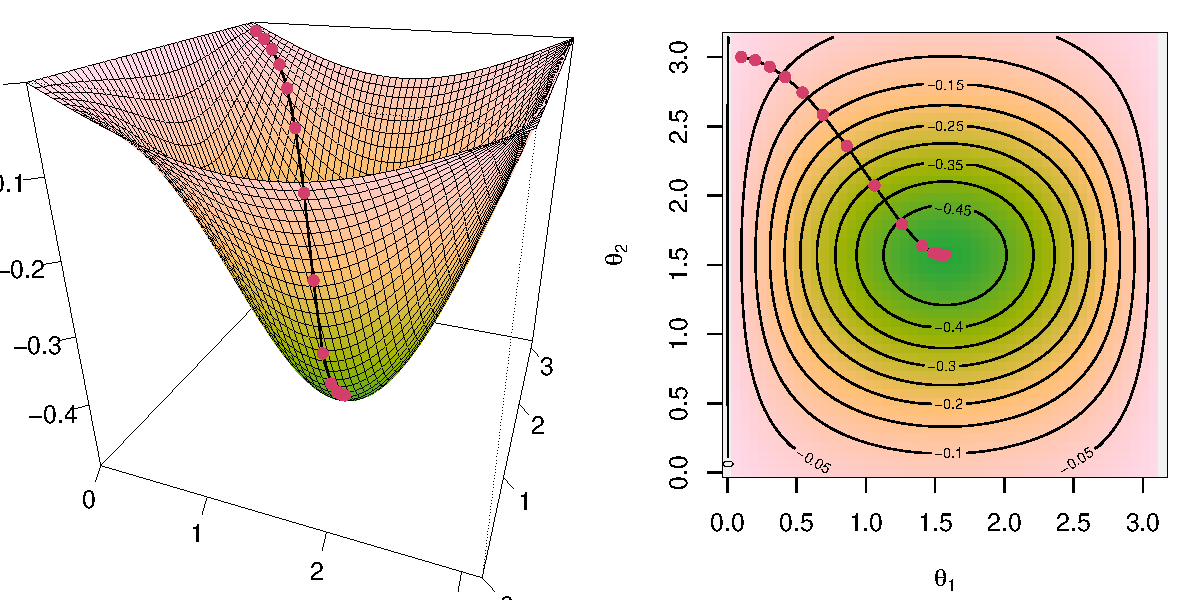
\includegraphics{figure_man/hill.pdf}}
\end{figure}
\vspace{1 cm}
"Walking down the hill, towards the valley."
\end{center}
\end{vbframe}
%%%%%%%%%%%%%%%%%%%%%%%%%%%%%%%%%%%%%%%%%%%%%%%%%%%%%%%%%%%%%%%%%%

\begin{vbframe}{Weight updates with Backpropagation}
\begin{itemize}
\lz
\item To update each weight $w \in \thetab$ in the network, we need their gradients with regards to the risk.
\lz
\lz
\item Since weights are stacked in layers inside the network, we need to repeatedly apply the \enquote{chain rule of calculus}. This process is called \textbf{backpropagation}.
\lz
\lz
\item After obtaining the gradients, the weights can be updated by GD:
$$\thetab^{[t + 1]} = \thetab^{[t]} - \alpha \cdot \frac{1}{n} \cdot \sumin \nabla_\theta L\left(\yi, f(\xi ~|~ \thetab^{[t]})\right)$$
\end{itemize}
\end{vbframe}
%%%%%%%%%%%%%%%%%%%%%%%%%%%%%%%%%%%%%%%%%%%%%%%%%%%%%%%%%%%%%%%%%%

\begin{vbframe}{Stochastic Gradient Descent}
\begin{itemize}
\lz
\item Optimization algorithms that use the entire training set to compute updates in one huge step are called \textbf{batch} or \textbf{deterministic}. This is computationally very costly or often impossible.
\lz
\item Instead of running the sum over the whole dataset (\textbf{batch mode}), one can run over small subsets (\textbf{minibatches}) of size $m$.
\lz
\item With minibatches of size $m$, a full pass over the training set (called an \textbf{epoch}) consists of $\frac{n}{m}$ gradient updates.
\lz
\item This stochastic version of the batch gradient is known as \textbf{Stochastic Gradient Descent} (SGD).
\end{itemize}
\framebreak
%%%%%%%%%%%%%%%%%%%%%%%%%%%%%%%%%%%%%%%%%%%%%%%%%%%%%%%%%%%%%%%%%%

An illustration of the SGD algorithm: on the left is GD and on the right is SGD. The black line depicts the averaged value of $\thetab$.

\begin{figure}
\scalebox{1}{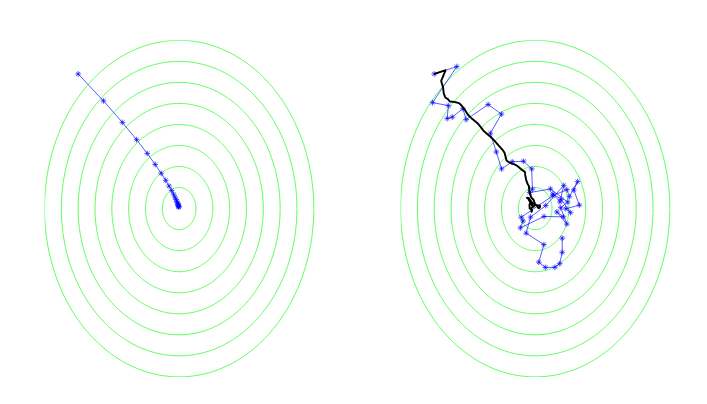
\includegraphics{figure_man/SGD.png}}
\tiny{\\ source : Shalev-Shwartz and  Ben-David.
Understanding machine learning: From theory to algorithms. Cambridge University Press, 2014.}
\end{figure}
\framebreak
%%%%%%%%%%%%%%%%%%%%%%%%%%%%%%%%%%%%%%%%%%%%%%%%%%%%%%%%%%%%%%%%%%

  \begin{algorithm}[H]
  \footnotesize
    \caption{Basic SGD pseudo code}
    \begin{algorithmic}[1]
    \State Initialize parameter vector $\thetab^{[0]}$
    \State $t \leftarrow 0$
    \While{stopping criterion not met}
    \State Randomly shuffle data and partition into minibatches $J_1, ..., J_K$ of size $m$
      \For{$k\in\{1,...,K\}$}
      \State $t \leftarrow t + 1$
      \State Compute gradient estimate with $J_k$:
      \[\hat{g}^{[t]} \leftarrow \frac{1}{m} \sum_{i \in J_k} \nabla_\theta L(\yi, f(\xi ~|~ \thetab^{[t-1]}))
      \]
      \State Apply update: $\thetab^{[t]} \leftarrow \thetab^{[t-1]} - \alpha \hat{g}^{[t]}$
      \EndFor
      \EndWhile
    \end{algorithmic}
  \end{algorithm}
\end{vbframe}
%%%%%%%%%%%%%%%%%%%%%%%%%%%%%%%%%%%%%%%%%%%%%%%%%%%%%%%%%%%%%%%%%%

\begin{vbframe}{SGD with Momentum}
\begin{itemize}
\item While SGD remains a popular optimization strategy, learning with it can sometimes be slow.
\item Momentum is designed to accelerate learning, by accumulating an exponentially decaying moving average of past gradients.
\end{itemize}
\begin{figure}
\centering
\scalebox{.8}{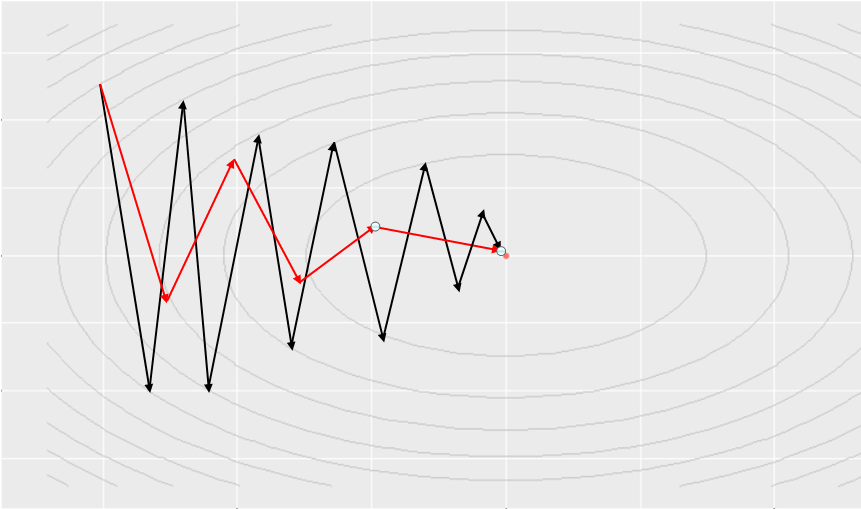
\includegraphics{figure_man/momentum.png}}
\\GD (black) versus momentum (red) when dealing with ravines
\end{figure}
\end{vbframe}
%%%%%%%%%%%%%%%%%%%%%%%%%%%%%%%%%%%%%%%%%%%%%%%%%%%%%%%%%%%%%%%%%%

\endlecture
\end{document}